\section{Background and Motivation} \label{sec:background}

What do people who talk about `comprehensible systems', `interpretable learning', `opaque systems', and `explainable AI' really care about? This paper tries to provide a more formal look at what components of a user's trust \edit{assurances for intelligent systems} would want to influence \edit{and how this can be practically accomplished by intelligent systems}. \nisarcomm{feels like more belongs here, specifically: an overview/summary of the main arguments and key takeaways from each of the following subsections in this section: a paragraph at this part should basically outline the skeleton of the key questions and ideas that the reader should be looking out for. Again, this can be written after the rest of the section itself is more solidified...}

\subsection{Motivation}
    Generally, humans have always wanted to trust the tools and systems that they create.  To this end many metrics and methods have been created to help assure the designers and users that the tools and systems are in fact capable of being applied in certain ways. \nisarcomm{and/or behave as expected; might also be worth mentioning here that `trust' is a fuzzy concept that will be defined more formally later on (help stave off lingering questions in reader's mind)}

    The situation has grown more complicated in recent years because the advanced capabilities of the systems that \edit{being created} can at times be difficult for even those who designed them to comprehend and predict. \edit{There are, for instance,} systems that have been designed to learn from extremely large amounts of data and expected to regularly perform on never before seen data. In some cases, such systems have been designed to perform tasks that might take humans entire lifetimes to complete. 

    Below is a small sample of some \edit{application} %research 
    areas that exist and a possible reason why they -- perhaps unknowingly -- have an interest in creating trustworthy systems.
    \nisarcomm{the application areas below are mostly OK [may want to trim/combine some], but your explanations of why trust matters feel weak and undifferentiated from each other. You might need to say a bit more about the potential risks/consequences or dangers/pitfalls of placing improper trust in each case, or why it is not necessarily obvious in any given area that algorithms are to be trusted, e.g. if something is `optimally' trained, then how come we can't say already say that it is actually `the best'? Or how do the needs of one particular area specifically impose different demands on trust than other areas?}
	% \begin{sidewaysfigure}[htbp]
        % 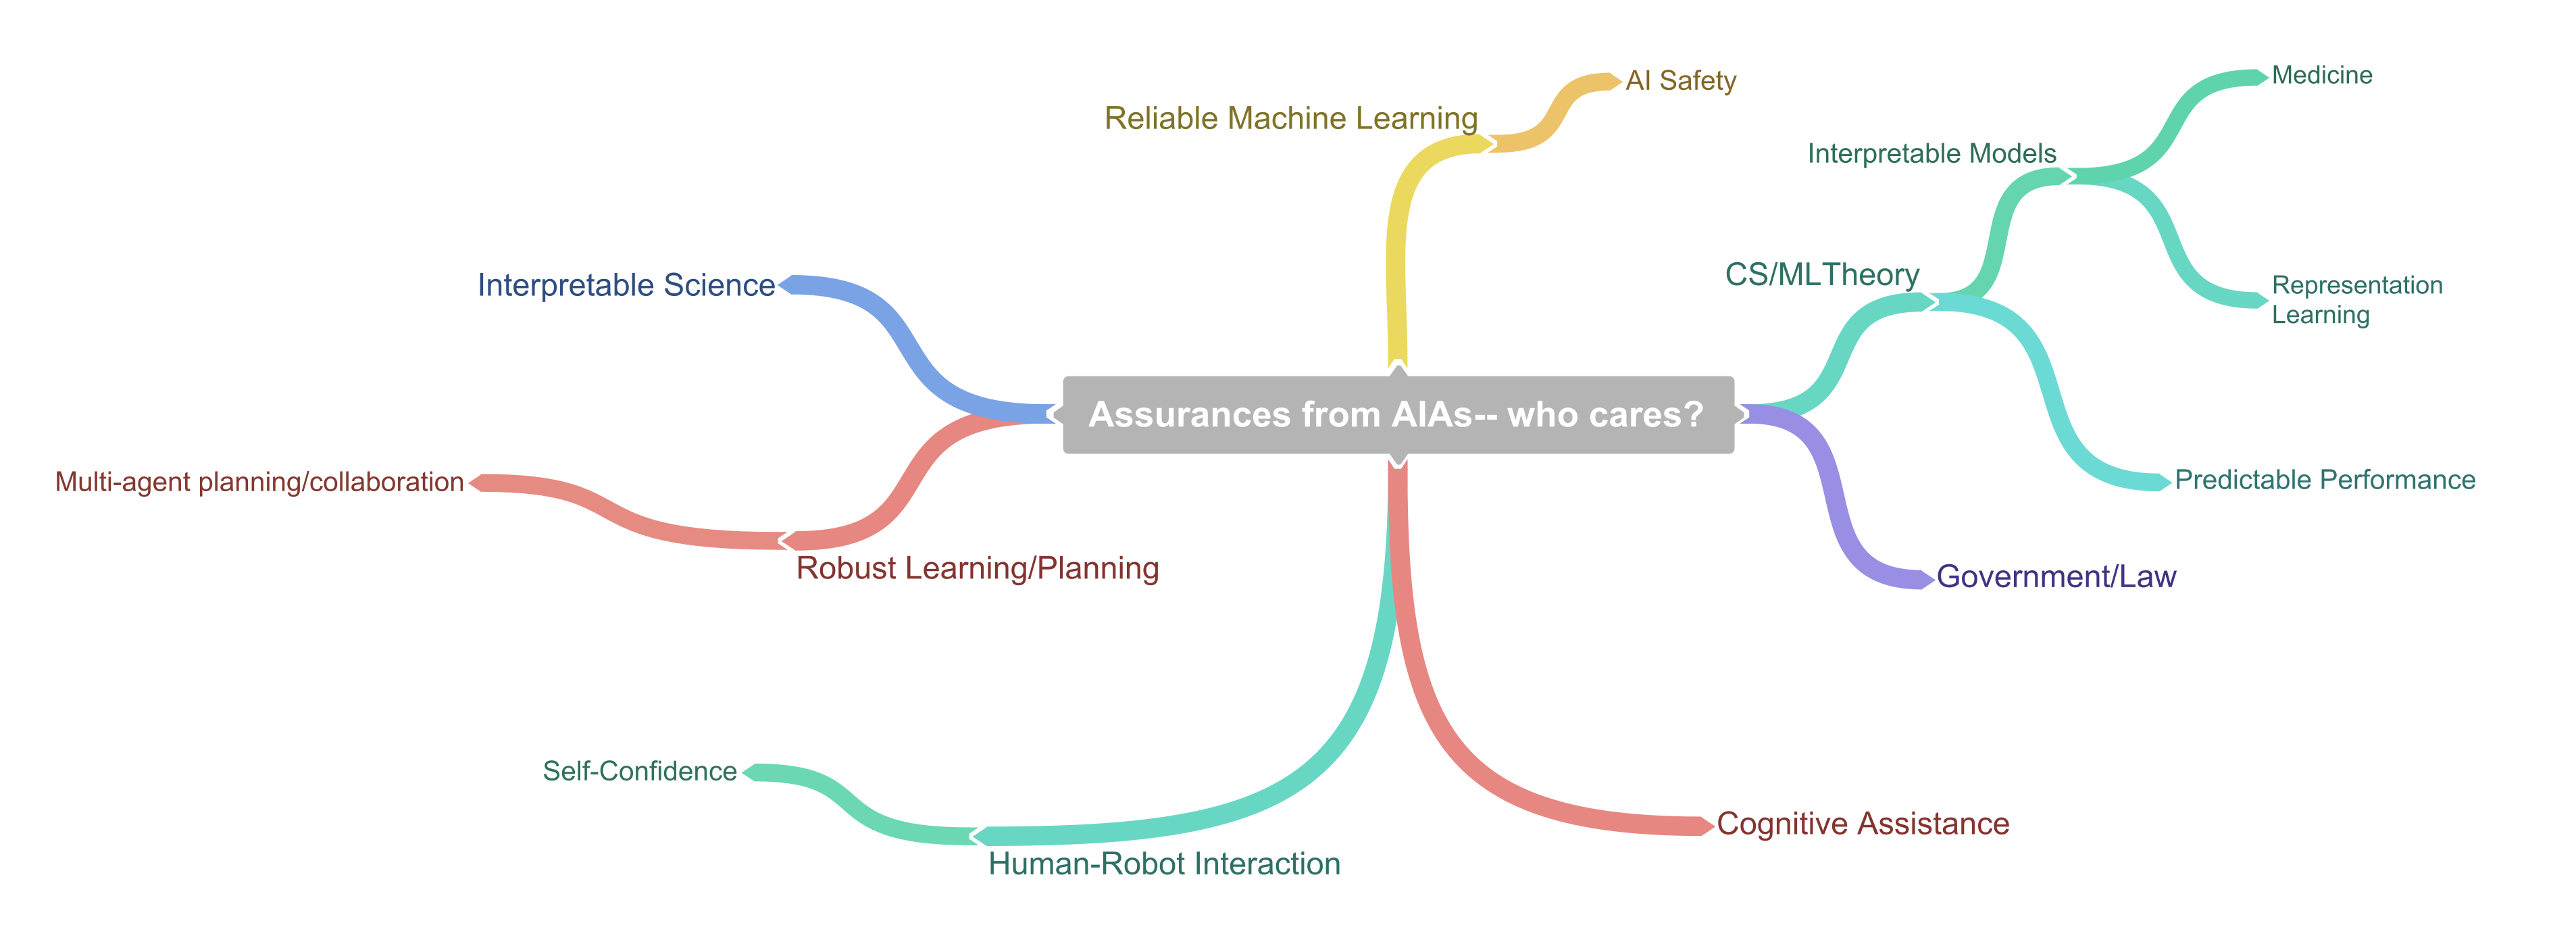
\includegraphics[width=7.5in]{Figures/WhoCares_cleaned}%
        % \caption{A diagram showing some of the academic disciplines that want to trust AIs more fully}
        % \label{fig:WhoCares}
    % \end{sidewaysfigure}
%
    \begin{description}
        \item [Interpretable Science:] Need to trust that the models created are valid, and be able to draw insights from them
        \item [Reliable Machine Learning:] Need to have safety guarantees for AIAs that have been deployed in real-world environments
        \item [Algorithms:] Need to trust how algorithms will perform on empirical data \nisarcomm{this is unclear -- clarify what this means; how is `algorithms' different than reliable ML or AI/ML?}
        \item [AI/ML:] \nisarcomm{define acronyms} Interpret how/why theoretical models function, to be able to trust them to function properly \nisarcomm{still kind of vague, clarify or be more precise }
        \item [Government:] Regulations on the interpretability of certain algorithms \nisarcomm{again very vague -- doesn't sound different from what you have above}
        \item [Cognitive Assistance:] Need to trust and understand recommendations given by automated personal assistants
        \item [Medicine:] Understand why data-driven models give predictions so that the predictions can be safely followed
        \item [HCI:] Help humans and computers interact in a more natural way, this involves finding ways for humans to trust computers more fully \nisarcomm{this feels like a rather broad category: is cognitive assistance not a part of HCI? } 
    \end{description}

    Revisiting a key point from the introduction, humans want to design assurances to help them appropriately trust AIAs. There are a few research fields that have formally and explicitly considered trust between humans and technology. Some examples are: e-commerce, automation, and human-robot interaction. However, due to their main goals they have not focused on explicitly designed assurances that affect trust, rather they studied implicit properties of systems that affect human trust.

    Conversely, there are other research fields that have informally considered how to affect the trust of designers and users using explicitly designed assurances. \edit{However,} due to their informal treatment of trust, it is unknown and unclear how effective these designed assurances might be, \edit{or what principles ought to be considered when designing assurances for general AIAs}.

    \subsubsection*{Survey Methodology} \label{sec:methodology}
    While theoretically a two-way trust model could be considered (i.e. in which the AIA also has trust in the user), attention is restricted here to a one-way trust relationship that considers only how user trust (and TRBs) evolves in response to assurances from the AIA. 

    It should be noted that it is practically impossible to perform a fully comprehensive survey of all AIA assurances, due to the broad spectrum of possible assurances, and AIAs in general. As an example, one could rightly argue that control engineers treat metrics like gain and phase margins as assurances for automatic feedback control systems, in much the same way that machine learning practitioners treat training and test accuracy as assurances for learning algorithms---and hence concepts related to robustness, stability, etc. for feedback control systems ought also be included in this survey. Similar arguments for assurances developed for fields like econometrics, software testing, aeronautical engineering and many others. While assurances can, in theory, be applied in both the most simple `automatic' systems (like a thermostat), this survey will focus on assurances in more advanced AIAs that make decisions under uncertainty. However, the admittedly narrow scope of this survey does not impede the development of fundamental insights and principles in designing assurances.

    Initially, in order to find applicable research, papers that formally addressed trust, and tried to create models of it, were investigated. This was done with the aim of trying to understand how trust might be influenced. Secondly, literature regarding trust between humans and some form of machine entity was reviewed; this lead to research in fields like e-commerce, automation, and human-robot interaction. Third, research on `interpretable', `comprehensible', `transparent', `explainable', and other similar types of learning and modeling methods were examined. Finally, with that literature as a background, research disciplines investigating computational methods that can be useful as assurances, but in which trust itself is not the main focus, were considered. This information was then used to construct an informed definition and classification of assurances based on methods that are currently in use, or being investigated.
    
    We now proceed to discuss each of the categories from Figure~\ref{fig:assurance_continuum}, starting from the most integral to the AIAs core functionality and proceeding to the least integral.


\subsection{Related Work}
    \citet{Lillard2016-yg} addressed the role of assurances in the relationship between humans and autonomous systems, \edit{and provides much of the foundation for describing the relationships between assurances and trust in human-AIA interaction}. 
%    . This paper is clearly related. 
Here, the assurance framework is presented in a way that is both more general and more detailed, albeit with the same end goal of being applied in a \edit{very similar end application}. \nisarcomm{BUT YOU NEVER SAY OR DEFINE/DESCRIBE WHAT THIS END APPLICATION IS!!!!! } 
\edit{For instance}, instead of \edit{assuming} that the user-autonomy trust loop is very strict and well structured, and that user trust does not take into account the institutional component proposed by \citet{McKnight2001-fa}, we \edit{account for} the notion of institutional trust in  human-autonomy relationships. \nisarcomm{at this point, I think reader/audience will be a bit frustrated by your extremely loose and inconsistent use of `autonomy' vs. `AIA' in phrases like `human-autonomy relationships' -- I think you ought to pick one and stick with it consistently throughout. Otherwise, be more explicit and clear up front which kinds of human-AIA systems *you* actually care about moving forward (i.e. human-autonomous vehicle systems), and then take care to mention why you are looking at more general types of AIAs instead of just focusing on autonomous vehicles (this relates to the point (ii) above: autonomous systems are relatively new, and you are looking at other AIAs to get at the core principles and insights for design of assurances)}

    Regarding the relationship with the work of \citet{McKnight2001-fa}, who made a typology of interpersonal trust,  we adopt the position that besides being applied to the e-commerce industry their trust model also applies to relationships between humans and AIAs (as in \citet{Lillard2016-yg}). However, here it is argued that assurances cannot directly have an affect on the user \edit(trust-related behaviors) TRBs \nisarcomm{avoid McGuire-ing here: DEFINE the acronym before using it -- don't assume that reader has seen it in the text -- some readers will skip past figure and thus not know what this means}. 
    The premise is that no autonomy (or vendor) should be able to control the TRBs of a human.

    The contributions of this work are to illuminate the connection between general AIA capabilities and general user trust. To classify assurances. To suggest that TRBs need to be calibrated \emph{not} trust. \textbf{add more here} \nisarcomm{not sure what last sentence means??}

\textbf{\nisarcomm{ would strongly recommend that you provide simple `operational' definitions for AIA, trust, assurances, TRBs at beginning (with a contextual/concrete example of each, say in the context of the road network application) and then explain methodology, and THEN dive into each component more as you have in different subsections -- rather than waiting until after describing your methodology to first define each term separately, and then providing in depth definition for each, without any contextual example at all to guide/frame the discussion. The methodology is hard to follow without having any kind of simple definition or understanding of why each component matters, and your readers won't really get where you're going with all of this.}}

\subsection{Artificially Intelligent Agents} \label{sec:aias}
    Intelligent technology spans a wide spectrum of capabilities. With regards to autonomous systems, these might include anything from a thermostat, to the fabled HAL 9000. While the main interest of the authors is geared towards human trust in `advanced' technology, this survey we will take a more holistic view and use the term \textit{Artificially Intelligent Agent (AIA)} to encompass a broad range of technologies that can be considered `autonomous'. This is done in order to provide generally applicable definitions and insights. 

    To this end, an artificially intelligent system needs to possess at least some of the capabilities shown in Figure~\ref{fig:AIcapabilities}~\cite{Russell2010-wv,Nilsson2009-rp,Luger2008-vf}. Some might argue that it is also necessary to add other categories like creativity and social intelligence~\cite{Tao2005-kh}. 
    \brettcomm{SEEMS TO DETRACT---}Some of these categories are also not clearly separable; for instance, where does the capability to `plan' end, and `reasoning' begin? Nevertheless, these capabilities are conceptually useful in defining an AIA:     
    \begin{description}
        \item[Artificially Intelligent Agent (AIA):] an agent that acts on an internally/externally generated goal, and possesses, to some extent, at least one of the capabilities shown in Fig.~\ref{fig:AIcapabilities}.
    \end{description}

	\begin{figure}[htbp]
    	\centering
     	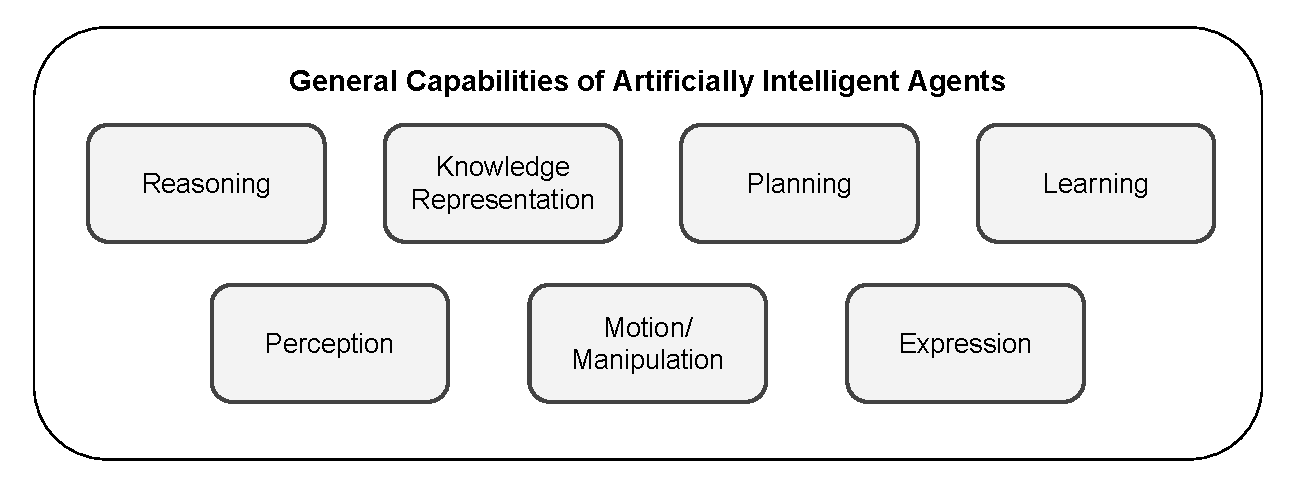
\includegraphics[width=0.55\textwidth]{Figures/AI_capabilities}
    	\caption{List of possible AIA capabilities.}
        \label{fig:AIcapabilities}
    \end{figure}

    The broad range of AIAs implied by this definition is most usefully viewed in terms of scope and adaptability. Scope refers to the range of possible applications for an AIA: does it have a small number of specialized application, or can it be used in many different applications? Adaptability refers to the ability of the AIA to become better at executing its goal over time. Low adaptability has often been associated with `weak AI' whereas high adaptability is often associated with `strong AI'.  Figure~\ref{fig:StrongWeak} depicts these axes for some (real and fictitious) AIAs.

	\begin{figure}[htbp]
    	\centering
     	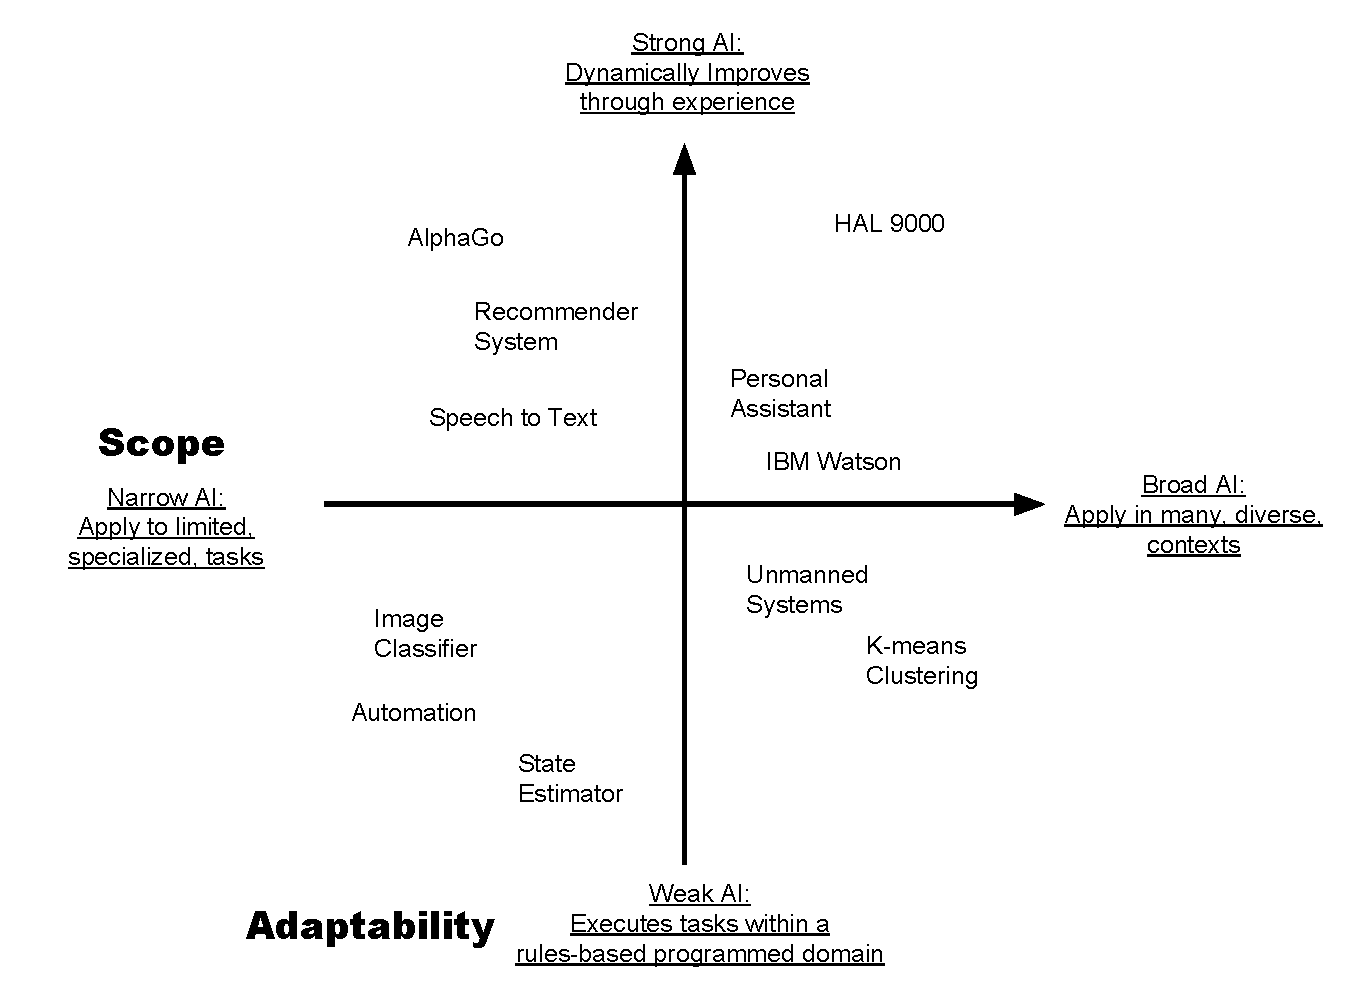
\includegraphics[width=0.7\textwidth]{Figures/strong_weak_narrow_broad.pdf}
    	\caption{Illustration of the range of systems encompassed by the AIA definition. Horizontal axis reflects the scope of the AIA, the vertical axis reflects the adaptability of the AIA.}
        \label{fig:StrongWeak}
    \end{figure}

    Arguably, we might instead have used the term `artificial intelligence' (AI) instead of AIA. However, `AI' carries too much ambiguity (in its fullest meaning, it would possess all capabilities from Figure~\ref{fig:AIcapabilities}, and more). AIA allows the broad inclusion of \emph{any} system in the adaptability/scope plane. The research discipline of machine learning (ML) is a subset of the AI research landscape. Individual ML algorithms might be thought of as being a narrowly scoped AI that is contained within only one of the AIA capabilities. 

    One might also question the need to define AIAs in the first place. This is to aid in the search for and understanding of assurances. As will be shown later, different methods of assurance can be found over the entire range of AIAs, so that an automation system such as a factory robot might be able to use similar assurances -- or more generally, similar principles of assurance -- as might a self-driving car, and vice-versa. The capabilities of AIAs (Fig.~\ref{fig:AIcapabilities}) are the sources of assurances; in other words, assurances cannot exist without some grounding set of AIA capabilities. 

    This definition, while broad, is still useful because it encompasses many of the systems that are typically described as `artificially intelligent'. More importantly, many of the assurances that exist for the simplest AIAs (e.g. chi-square consistency tests for a Kalman filter state estimator) can be adapted/generalized for use in more advanced AIAs. In other words, the proposed definition of AIAs sets an \emph{appropriate scope} for the bodies of research that are likely to have investigated assurances and assurance principles that can be generalized/extended to any intelligent computing system. The definition of AIAs and their range of capabilities also helps to understand and establish what kinds of assurances might be needed in future systems. For example, assurances from an AIA that can only carry out planning tasks will probably differ in design and/or application from assurances from an AIA that can only carry out perception tasks. 

\subsection{User Trust} \label{sec:trust}
    In designing assurances, which affect trust-based user behaviors, it is critical to know what drives those behaviors. Because of this, some time must be spent to understand what trust is. 

    Trust is critical in interpersonal relationships, and it affects the dynamics of \edit{intelligent multi-agent} systems as simple as \edit{one-on-one personal interactions}  \cite{Lewicki2006-hj}, to more complicated ones such as financial markets and governments \cite{Fukuyama1995-un}. Consequently, researchers in psychology, sociology, and economics have historically sought to understand the fundamental principles of trust, each with the aim of understanding their field better \cite{Gambetta1988-pi}. Moral philosophers have also thought intently about the topic \cite{Baier1986-im}.

    Due to wide interest spanning many disciplines it is difficult, if not impossible, to write a succinct definition of trust that would appease all interested parties. Besides that, trust is actually a very broad concept that evades precise definitions at a high level. However the following definition, adapted from \cite{McKnight2004-vv}, is broad enough to avoid too much contention:

    \begin{description}
        \item [Trust:] \edit{a psychological state in which an agent} willingly and securely becomes vulnerable, or depends on, a trustee (e.g., another person, institution, or an AIA), having taken into consideration the characteristics (e.g., benevolence, integrity, competence) of the trustee.
    \end{description}

    \subsubsection{Trust in AIAs and humans?}
        Trust is generally understood to exist between people. Is it possible for a human to enter into a trusting relationship with an AIA?
        % In their paper regarding important human factors that should be considered when designing autonomous machines \cite{Sheridan1984-kx} are seemingly the first to discuss the idea that trust relationships between humans and autonomous systems are important, and to suggest that humans need some assurance that the ``commands will be carried out properly''. They also mention the idea that ``there needs to be an accurate perception of [the autonomous system's] trustworthiness''. Finally they suggest that ``appropriate criteria for trust need to be studied to develop a theory of trust in supervisory control''.
        % Perhaps motivated by \citeauthor{Sheridan1984-kx}\cite{Sheridan1984-kx}, a few years later \cite{Muir1987-mk}, and later in more detail \cite{Muir1994-ow}, create a psychologically based model of trust that considered the ``component expectations of trust'' of \cite{Barber1983-yc} and the dynamic evolution of trust from \cite{Rempel1985-sg}, to make a framework for studying trust in human-machine relationships.
        % \citet{Muir1996-gt} reported the results of two experimental studies to investigate the validity of her proposed model. She claims that these were the first experiments to explicitly ask "operators to rate their trust in automated equipment", and to see if they could do so under normal operating conditions. She found that operators were able to rate their trust in the automation, and that the level of trust changed based on different performance characteristics of the automated system. In her own words: "These results suggest that operators' subjective ratings of trust and the properties of the automation which determine their trust, can be used to predict and optimize the dynamic allocation of functions in automated systems".
        That humans actually do feel trust towards machines has been experimentally confirmed several times in research using common subjective psychological questionnaires. Some examples include: \citet{Muir1996-gt,Reeves1997-ad,Groom2007-bz,Mcknight2011-gv,Riley1996-qm,Bainbridge2011-pl,Kaniarasu2012-mo,Salem2015-md,Desai2012-rc, Freedy2007-sg, Wang2016-id, Inagaki1998-cl, Kaniarasu2013-ho}. 
\nisarcomm{This next part is worth mentioning:} Several academic experiments have investigated the possibility of trust existing between humans and (according to the terminology of this survey) AIAs. All found that some level of trust can be formed in such relationships. For instance, ref. \citet{Lacher2014-yc} points out that people trust an AIA at different levels. For example, an operator would have different perspectives on trust based on their level of interaction with the AIA. The designer of an AIA would also trust the AIA differently than an end user, due to the differing nature of the trust relationship from one to the other. 
        % \citet{Lankton2008-ct} claims, and finds some support for the idea, that trust in technology is fundamentally different from interpersonal trust between humans. They demonstrate the validity of the hypothesis by using a survey of 427 college students regarding Facebook. However, the authors point out that this study was based on a single set of survey data about facebook, and may not be unbiased or apply to other technologies. Beyond this, it is the author's opinion that the `fundamental differences' they point out are not that divergent from the human-human trust model.

        Ref. \citet{Tripp2011-cq} investigate the variation of trust between humans and different levels of technology. They run experiments with three different levels of technology: Microsoft Access, a recommender system, and Faceobook. They found that `human-like' trust applied more to Facebook, while `system-like' trust applied more to MS Access. They conclude that if the system is `human enough', then a human trust model is appropriate. However, the authors also caution that it is important to check first \nisarcomm{Check what first???}.

        Given this research, we will take the position of presenting a human-human trust model and using it as a basis for human-AIA trust -- with the understanding that the applicability of the model varies with the complexity of the AIA. For example, something in the lower-left quadrant of \ref{fig:StrongWeak} \edit{?????} to the upper-right quadrant. \nisarcomm{CAREFULLY READ ALOUD WHAT YOU ARE WRITING: (i) previous sentence is a sentence fragment, and (ii) also this seems like a very strange thing to say: you are applying a human-human trust model as basis for all human-AIA trust, but then you are immediately disclaiming that it is not really applicable in all AIA cases? Then why bother presenting it?! Are you really trying to say something else here, i.e. some features of the model may be more important than other features depending on where you are on the spectrum of adaptability vs. capability? }

\subsubsection{A Model of Human-AIA Trust}
We now present a model of human-AIA trust, which will cast insights on assurances that will be discussed later. It should be noted that this model is being presented as \emph{one possible model} that can be helpful in understanding assurances -- it is neither the only model nor a perfect model. As research advances, such models will also likely continue to evolve, and the ideas of assurances will naturally evolve as well.
        % This has been recently attempted in the context of human-AIA relationships \cite{Lahijanian2016-nd}, but with an overly simplistic reduction of trust. The reality is that trust is extremely complex, and so dealing with it in the setting of human-AIA relationships is going to be complex.

In work relating to business management, McKnight in ref. \citet{McKnight1998-ty} and later in ref. \cite{McKnight2001-fa} performed what is, arguably, the first multi-disciplinary survey and unification of trust literature, which also condensed it into a single typology. The resulting model is shown, with some minor adaptations, in Figure \ref{fig:UserTrust}.

        \begin{figure}[htbp]
            \centering
            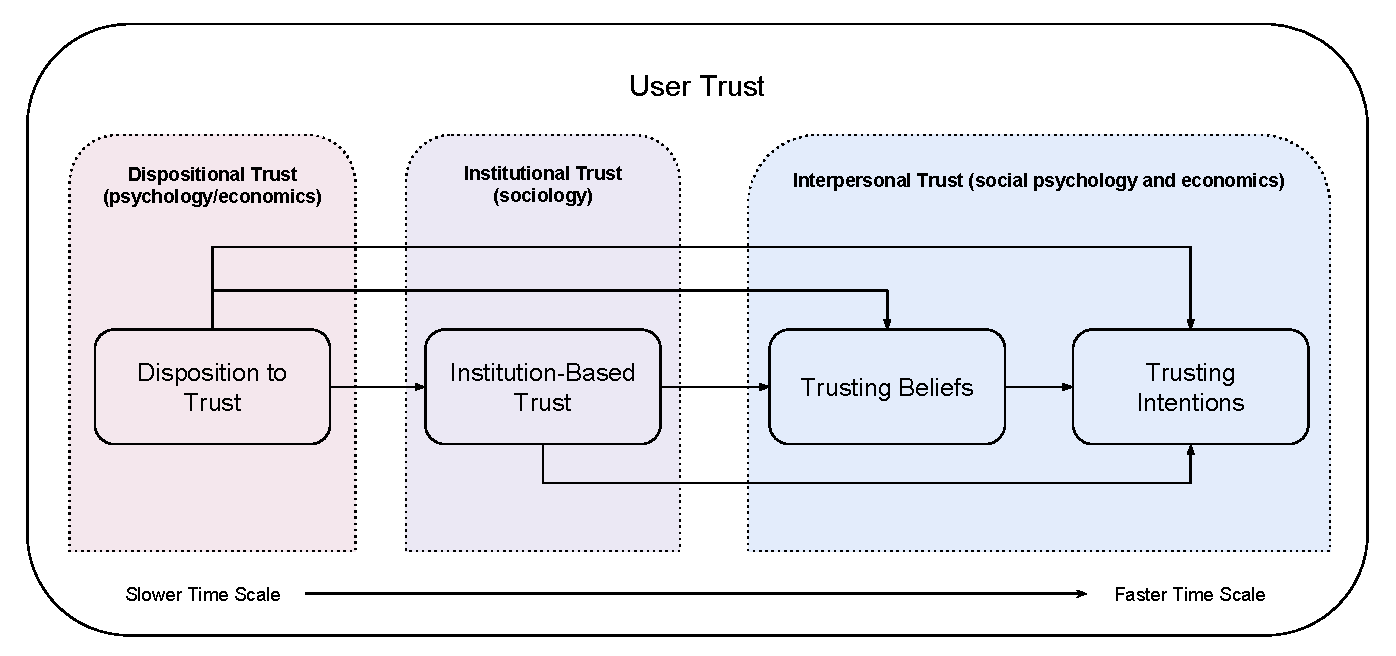
\includegraphics[width=0.9\textwidth]{Figures/UserTrust}
            \caption{Interdisciplinary trust model proposed by \citet{McKnight2001-fa}. The three main categories are delineated, and corresponding disciplines that are interested are listed within parentheses. Connections indicate a causal relationship.}
            \label{fig:UserTrust}
        \end{figure}

        The categories \nisarcomm{of what??} are defined as follows: \nisarcomm{You jumped into the figure without describing anything about it at a high level at all!!! What categories are you talking about -- categories of WHAT exactly??? SAY what the figure means at a high level -- walk the reader through it so they are on the same page as you -- \textbf{DON'T WRITE TO YOURSELF, WRITE FOR YOUR AUDIENCE (WHICH HAS NOT YET SEEN WHAT YOU HAVE SEEN) -- PUT YOURSELF IN AUDIENCE'S SHOES}}

        \begin{description}
            \item [Disposition to Trust:] The extent to which one displays a consistent tendency to be willing to depend on others (and AIA) in general across a broad spectrum of situations and persons
            \item [Institution-Based Trust:] One believes that regulations are in place that are conducive to situational success in an endeavor
            \item [Trusting Beliefs:] One believes that the AIA has one or more characteristics beneficial to oneself
            \item [Trusting Intentions:] One is willing to depend on, or intends to depend on, the AIA even though one cannot control its every action
        \end{description}

        Each of these main categories \edit{of trust} has components defined in Figure \ref{fig:Assurance_classes}. These components were defined through the compilation of many research studies across research disciplines, and because of this represent the most accurate notion of the components of trust available. \edit{It is asserted here} that these trust components \hlr{describe the possible dimensions that constitute trust-related behaviors} \nisarcomm{this is not worded correctly -- these are components of trust, not trust-related behaviors -- they might inform TRBs, but they are not in and of themselves things that constitute TRBs (which you have yet to define at this point!)}, and at which assurances \hlr{must be} targeted. \nisarcomm{MUST be targeted? or are targeted? i.e. is there any real choice? }

        \begin{sidewaysfigure}[htbp]
            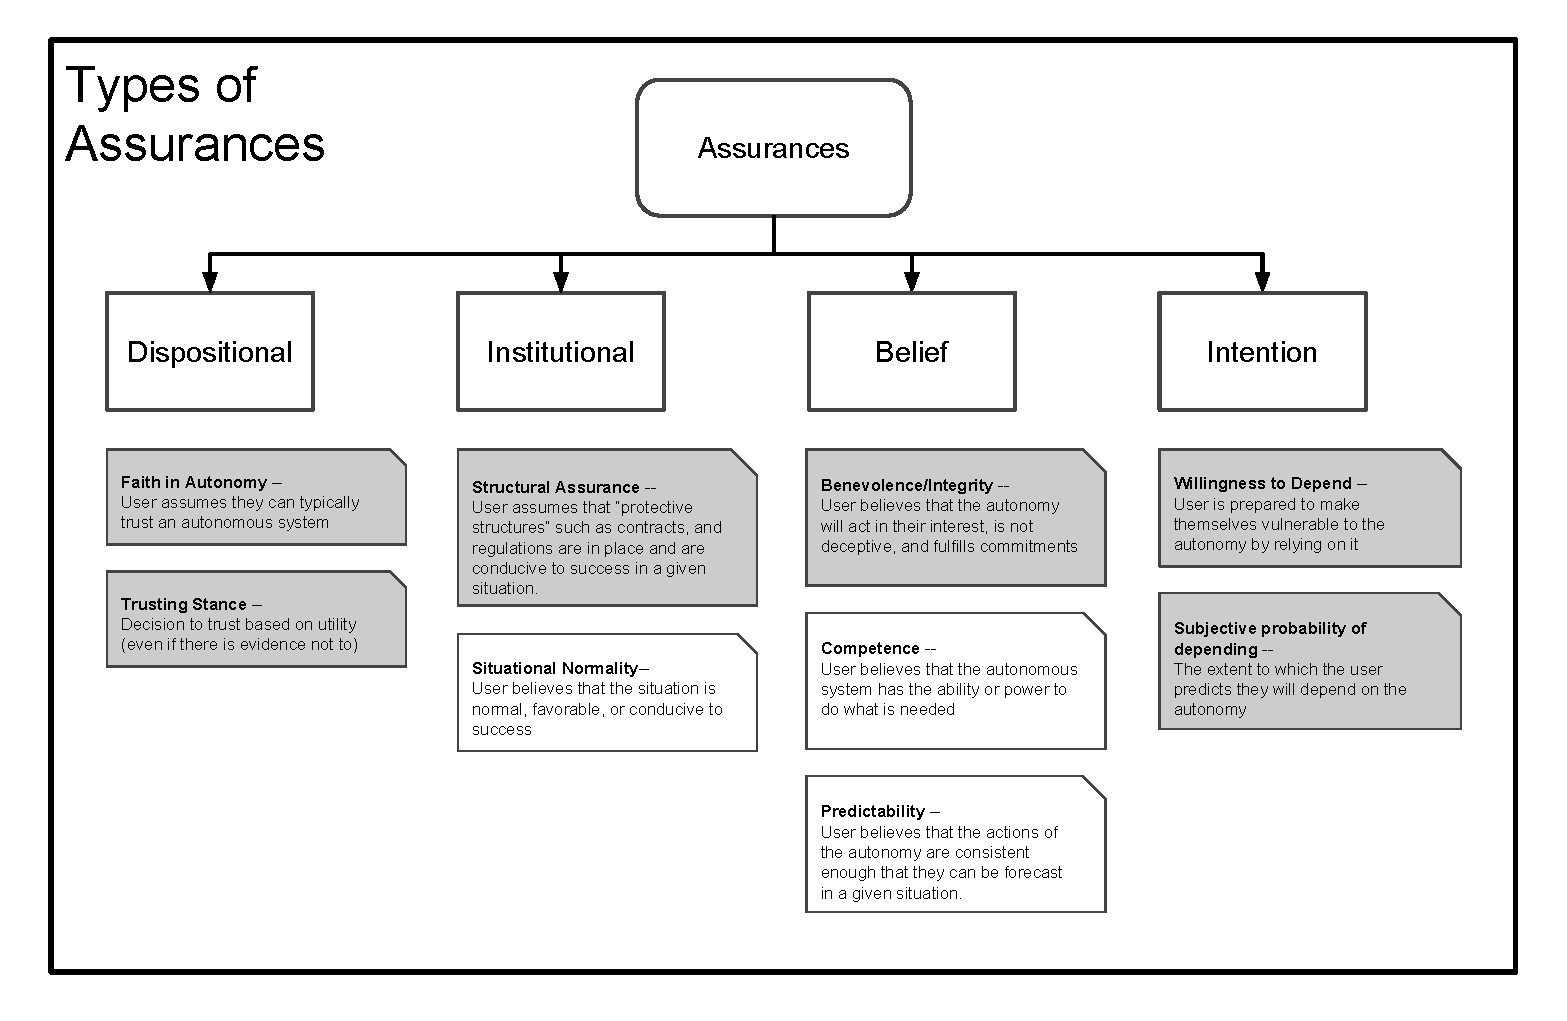
\includegraphics[width=8in]{Figures/Assurances.pdf}%
            \caption{\textbf{Diagram delineating the possible classes of assurances, and suggesting those classes that directly apply in calibration of TRBs \ldots obviously needs to be finished \ldots}}
            \label{fig:Assurance_classes}
        \end{sidewaysfigure}

%trbs.tex
%\nisarcomm{trim, merge, move earlier?....}

%Researchers of all disciplines widely accept that 
Trust ultimately leads to some kind of meaningful behavior or action which reflects the level of trust \cite{Lewis1985-pr}. 
%; this idea was highlighted by \citet{Lewis1985-pr}.  
These are called `trust-related behaviors' (TRBs) \cite{McKnight2001-fa}. %, which is the term that will be used in this survey. 
In the case of a human-AIA relationship per Fig. \ref{fig:SimpleTrust_one_way}, %and \ref{fig:RoadNet}, 
Some example TRBs could include the kinds of tasks the human user assigns to the AIA, accepting and following through on a plan produced by the AIA, or directing that a new plan be made, or switching off autonomous capabilities altogether to teleoperate and perform tasks manually through a physical mechanism that the AIA otherwise controls.  %the vehicle. 

%\subsubsection{Calibration of Trust-Related Behaviors}
    
    Trust is not a univariate quantity that can be objectively measured. Rather, it is a multidimensional phenomenon whose `relative magnitudes and directions' must be observed through changes in TRBs, or qualitative self-reports reported in surveys \cite{Muir1996-gt}. It thus comes as no surprise that TRBs are the more objective measure due to the fact that people are not always consistent in their ratings, and may sincerely feel different levels of trust while performing similar TRBs. \citet{Parasuraman1997-co} were interested in understanding the use of automation by humans, and defined terms to describe that use. Here it is proposed that, by extension, those terms also apply to the behaviors of humans towards more advanced AIAs. Within this scope the definitions are as follows: \textit{Misuse:} over-reliance on an AIA (which could manifest itself in a user's unrealistically optimistic expectations of performance); \textit{Disuse:} under-utilization of an AIA (e.g. a user turning off the AIA, or failing to use all of its capabilities); \textit{Abuse:} Inappropriate application of an AIA (where \emph{application} in this case means the choice to deploy an AIA in a certain context).

    \nisarcomm{can trim down this parag a bit...}
    Following Fig.~\ref{fig:SimpleTrust_one_way}, an AIA's assurances are ideally designed to steer the user away from misuse, disuse, or abuse of the AIA, i.e. towards otherwise appropriate TRBs. This can only be done by properly `calibrating' assurances to suitably influence user trust. This is a point that, to some extent, has been informally mentioned in \cite{Muir1994-ow,Lillard2016-yg,Lee2004-pv,Hutchins2015-if}. Note that other researchers who propose `calibration' (or other similar concepts) often suggest calibrating \emph{trust} as opposed to TRBs. \citet{Dzindolet2003-ts} found that providing system performance feedback tended to increase user's \textit{self-reported trust}, even though user's resulting TRBs did not reflect self-reported trust levels. This shows the danger of calibrating `trust', as opposed to calibrating the TRBs. 
    TRB calibration focuses on concrete and measurable behaviors that are universally applicable. 
    In contrast, trust calibration involves influencing a quantity that is directly immeasurable, and that, when measured indirectly, is subject to individual human differences and biases. 
\subsection{Assurances} \ref{sec:assurances}
    The term assurances was introduced in the previous section as the name by which feedback will be known in a human-AIA trust relationship. As assurances are the main topic of this paper, and are have received very little attention in trust literature, a more detailed definition and discussion is merited.

    \citet{McKnight2001-fa} allude to this kind of feedback in an e-commerce relationship as `Web Vendor Interventions' and mention some possible actions that might be used in that specific application. They go as far as making a diagram that indicates that these interventions could affect the `Trusting Beliefs', `Trusting Intentions', and `Trust-Related Behaviors' (see Figure \ref{fig:UserTrust}).

    \citet{Corritore2003-gx} refer to assurances as `trust cues' that can influence how online users trust vendors in an e-commerce setting. \citet{Lee2004-pv} discuss `display characteristics', which are methods by which an autonomous can communicate information to an operator.
    
    The term assurances is perhaps earliest used in the context of human-automation relationships by \citet{Sheridan1984-kx}. More recently, and formally, \citet{Lillard2016-yg} defined the term `assurance', I extend the definition to be more general
    
    \begin{description}
        \item [Assurance:] A property or behavior of an AIA that affects a user's trust. As used here, the term is not intended to have a positive or negative connotation -- assurances can decrease trust.
    \end{description}

    Most familiar with the fields of AI, ML, data science, and robotics will recognize terms like \emph{interpretable}, \emph{comprehensible}, \emph{transparent}, \emph{verified and validated}, \emph{certified}, and \emph{explainable AI}, with respect to the models or performance of a designed system. A key claim of this paper is that from a high level all of these terms have the same aim: for a user to be able to trust an AIA to operate in a certain way, and based on that trust behave appropriately towards the AIA. Those actions might include re-design, as well as adjusting TRBs.
%
    % Assurances and `interpretability' are delicately linked. In fact, interpretability would be classified as one embodiment of an assurance. This relationship is highlighted by \citet{Vellido2012-nm} where they illustrate that interpreting an AIA is part of the knowledge discovery process.

    The sections that follow outline different classes of assurances.

    \subsubsection{Source-Target Classification}
    It is convenient to refer to assurances by way of their source and target. Intuitively, there may be a set of different algorithms that are useful for making assurances that convey information about planning to the competence dimension of the user's trust. It is easier to refer to these assurances in terms of their source and target. So, for this example that class of algorithms would be the `planning-competence' class.
    
    Not only is this useful shorthand for communicating about the purpose of the algorithms, but it is useful in classifying the range of assurance algorithms that exist. There may also be a class of algorithms that span multiple source-target capabilities. For example there may be a kind of algorithm that can give a `learning-competence' assurance, as well as a `planning-competence' assurance.

    This is especially true since many of the AIA capabilities can overlap. Also, the effects of assurances cannot be guaranteed to affect only one trust dimension.

    Figure \ref{fig:Assurance_classes} shows the hierarchy of proposed assurance classes. The categories mirror those of the trust model proposed by \citet{McKnight2001-fa}, but with the emphasis on what an AIA has the ability to most readily influence (and consequently where most research is found). The boxes with the beveled corner identify and define the different classes of assurances. All classes are included here for completeness and generality. Although, while it is hypothetically possible for an AIA to influence a persons general `Trusting stance' given enough time\footnote{One might imagine an AIA that specifically speaks to the human about the benefits or drawbacks about trusting even though there might not be evidence to do so, similar to the role a counselor might play}, the gray boxes are not considered further in this survey, as practically no direct research exists in the realm of human-AIA relationships.

    \textbf{ugggg, this gets a little complicated, but it's not supposed to be}.

    \subsection{Component and Composite Assurances}
Assurances can be either component or composite. This was seen a little through the survey. The definitions are as follows:

\begin{description}
    \item [Component:] An assurance that originates from a single AIA capability source, and targets a single trust dimension target.
    \item [Composite:] The combination of more than one component assurance into a single assurance. 
\end{description}

\begin{figure}[!htbp]
    \centering
    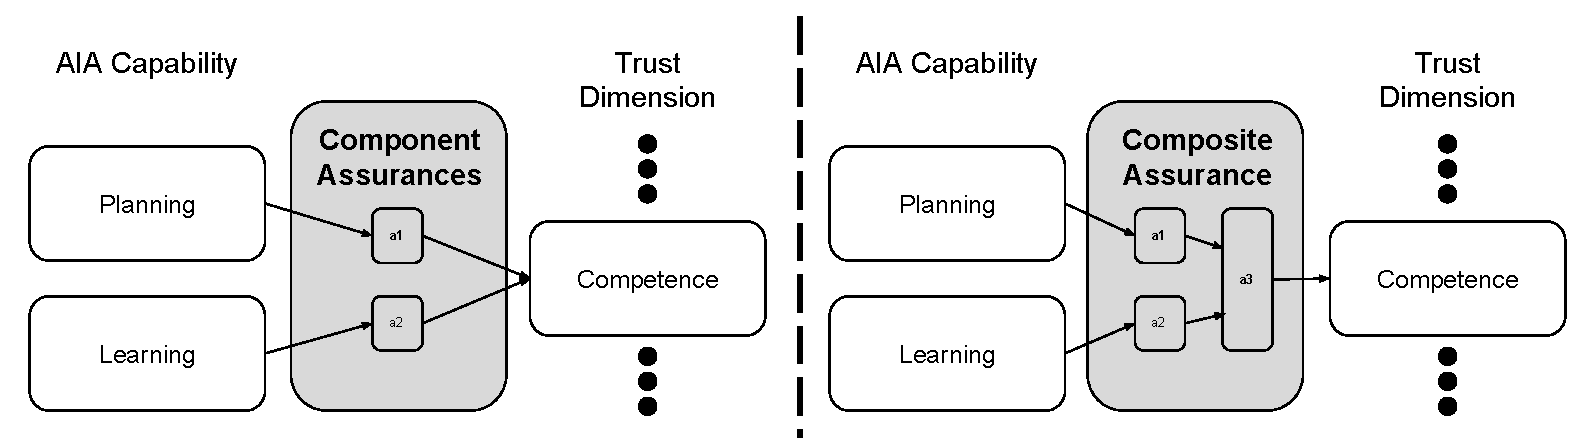
\includegraphics[width=0.9\textwidth]{Figures/Assurance_component_composite.pdf}
    \caption{Figure illustrating the difference between component and composite assurances. The existence of multiple assurances does not imply a composite assurances, rather the combination of multiple component assurances into a single assurance constitutes a composite assurance.}
    \label{fig:assurance_mapping}
\end{figure}

Figure \ref{fig:assurance_mapping} illustrates the concepts of component and composite assurances.

\paragraph{Component Assurances:} Component assurances are perhaps the most well researched in the existing literature. This is likely because several verified component assurances are the predecessors to composite ones. A component assurance might include displaying the confidence of a classification prediction, or visualizing a model as discussed in section \ref{sec:q2}.

\paragraph{Composite Assurances:} Composite assurances are assurances that are built of several components. A notable example is the work by \citet{Aitken2016-cv} who propose a measurement called `self-confidence', applicable to Partially Observable Markov Decision Processes (POMDPs). This metric combines five component assurances into a single composite assurance that is meant to distill the information into a value that a novice operator could understand easily. This paper was discussed in more detail in \ref{sec:q2}. 

    \emph{Tutoring vs Telling:}
Most assurances investigated to date are `telling', in that they do not consider the experience or other traits of different users. The ability to adapt to different users, and to tutor them to appropriate trust will become more critical as time passes due to the diversity of users bases for advanced AIAs and time that users will interact with them. A tutoring assurance would be a planned, dynamic, sequence of assurances that would change in time to adapt to the user's needs. This might include modification of assurances to help a user avoid boredom, or to use the system differently in varying circumstances. It isn't surprising that, to our knowledge, no research has been done with respect to tutoring a user in a trust relationship. This is a complex problem to address that would involve understanding how different users learn, and what an appropriate strategy would be to teach them to have appropriate TRBs. However, a rich resource (not investigated in this paper) would be the work on tutoring systems \citet{Wenger2014-ld} and algorithmic teaching \citet{Balbach2009-jw}.

    \subsubsection{Explicit and Implicit Assurances}
\citet{Sheridan1984-kx} briefly alluded to the existence of explicit and implicit assurances when they discussed the nature of how humans behave when working with automated systems. They suggested that the operator's perception of the automated system can be effected by `performance' and its `reports on its own performance'. 


\begin{description}
    \item [Explicit:] Assurances that are purposefully given to affect the trust of a user.
    \begin{itemize}
        \item Legible motion \cite{Dragan2013-wd}, which is motion calculated with the intent of being more understandable by a human
        \item $R^2$ value, gives some indication of how well the regression accounts for the variance of the data
    \end{itemize}
    \item [Implicit:] All other assurances that aren't explicit.
    \begin{itemize}
        \item Reliability in completing a task. Generally, the object of success is not to affect the user's trust (although this is a nice side-effect).
        \item The way an autonomous vehicle appears. For example something that looks neat will have a different effect on trust, than an AIA with wires dragging on the ground. 
    \end{itemize}
\end{description}




    \subsubsection{The \edit{Imprecise} Nature of Assurances}
        Due to the nature of trust (and humans in general), a single assurance might be targeted at influencing the competence dimension of trust, but it may also have effects on other dimensions. As an example an assurance aimed at influencing Predictability may also have an affect on the Probability of Depending.

        Besides being difficult to separate, each user is different. Thus no assurance will have an identical effect when given to two separate users. This makes it difficult to have precise effects on user trust behaviors.

        \textbf{I am not sure how I want this argument to go, I want to highlight that it is theoretically possible to have some affect on each of these attributes, but that some are more practical. Two main things need to be considred 1) time-scale (how long will it take to make a noticeable change), and 2) what SHOULD be influenced in order to appropriately calibrate TRBs (it probably isn't acceptable to lie in order to manipulate a user's trust)?}

